\chapter{設計と実装}
\label{chap:poordirection}

\section{提案手法}
本研究では,P2P型端末通信フレームワークであるAllJoynを用いて端末間のビーコン情報共有を行う.
具体的には,端末Aで周囲のビーコンを検知し,端末BにビーコンのUUID,RSSI,タイムスタンプなどの情報を送信する.
また,自身で検知したビーコンの情報と,他端末から送信されたビーコンの情報を保持する.
今回の設計では,同一アクセスポイント内に複数の端末があることを想定している.

\section{開発環境}
本研究では,対象OSをAndroidとし,Android OSで動作するアプリケーションを作成する.
なお,Android 4.3以上かつBluetooth4.0以上に対応した端末を想定している.
\begin{itemize}
\item 開発環境
\begin{itemize}
\item Eclipse 3.8 for Mac OS X
\item Android SDK Tools 23.0.5
\item AllJoyn Android v14.02
\end{itemize}
\item 使用端末
\begin{itemize}
\item TORQUEG01
\item ARROWS NX F-05F
\end{itemize}
\end{itemize}

使用した端末のスペックは以下の通りである.
\begin{table}[htbp]
\centering
\begin{tabular}{|c|c|} \hline
OS &  4.4.2 \\ \hline
CPU & MSM8928 1.4GHz クアッドコア \\ \hline
ROM & 16GB \\ \hline
RAM & 2GB \\ \hline
Bluetooth & Ver.4.0 \\ \hline
Wi-Fi & IEEE802.11a/b/g/n/ac \\ \hline
\end{tabular}
\caption{スペック:TORQUE G01}
\end{table}

\begin{table}[htbp]
\centering
\begin{tabular}{|c|c|} \hline
OS &  4.4.2 \\ \hline
CPU & MSM8974 2.3GHz クアッドコア \\ \hline
ROM & 32GB \\ \hline
RAM & 2GB \\ \hline
Bluetooth & Ver.4.0 \\ \hline
Wi-Fi & IEEE802.11a/b/g/n/ac \\ \hline
\end{tabular}
\caption{スペック:ARROWS NX F-05F}
\end{table}


\section{AllJoynAppの概要}
iBeaconから発せられるビーコンを受信し,AllJoynを用いてビーコン情報を送受信するAndroidアプリであるAllJoynAppを作成する.


\section{設計}
今回作成するAllJoynAppには,ビーコンを検知し,AllJoynを用いてビーコン情報を送信するAllJoynClientと,ビーコン情報を受信するAllJoynService,インターフェースを記述したSimpleInterfaceという三つのプログラムがある.
AllJoynServiceはバックグラウンドで動作するプログラムであり,AllJoynClientから呼び出されて起動する.
更に,FINDボタンとSCANボタン,ListViewといったUI部品がある.


\subsection{AllJoynセッション}
今回設計したAllJoynセッションの流れは以下の通りである.

\begin{figure}[htbp]
\centering
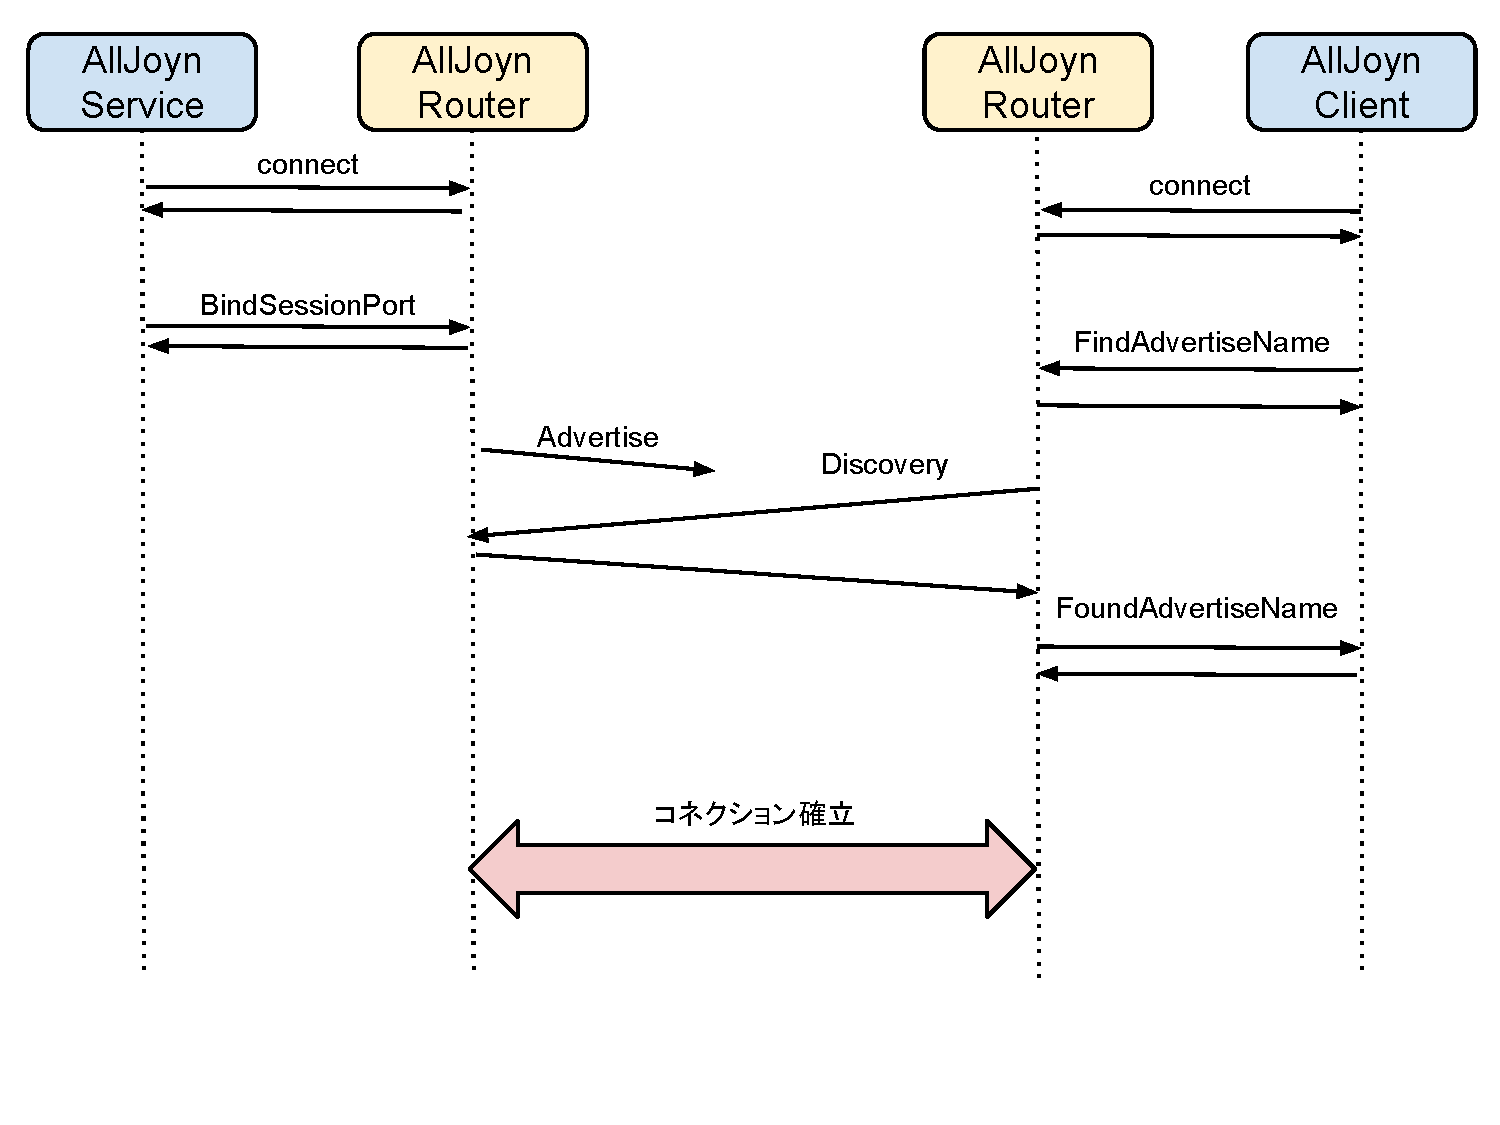
\includegraphics[width=10cm]{fig/AllJoyn_Session.pdf}
\caption{AllJoynセッションの例}
\end{figure}

\begin{enumerate}
\item AllClientとAllJoynServiceは,それぞれのAllJoyn Routerに接続する.
\item AllJoynServiceでは,BindSessionPort APIを用いてセッションポートやセッションオプションなどを決定する.
\item AllJoynServiceでは,AllJoyn Routerを通して任意の名前をAdvertiseしてコネクションを待つ.
\item AllJoynClientでは,AllJoyn Routerを通して任意の名前をDiscoverする.
\item Advertiseされている任意の名前と一致した場合,FoundAdvertiseNameシグナルがAllJoynClientに送られる.
\item AllJoynClientがJoinSession APIを用いてAllJoynClientとAllJoynServiceのコネクションが確立する.
\end{enumerate}


\subsection{プログラムファイル}
AllJoynAppは,
\begin{itemize}
\item AllJoynClient.java
\item AllJoynService.java
\item SimpleInterface.java
\end{itemize}
の三つのプログラムファイルから成る.


\begin{figure}[htbp]
\begin{minipage}{0.5 \hsize}
\begin{center}
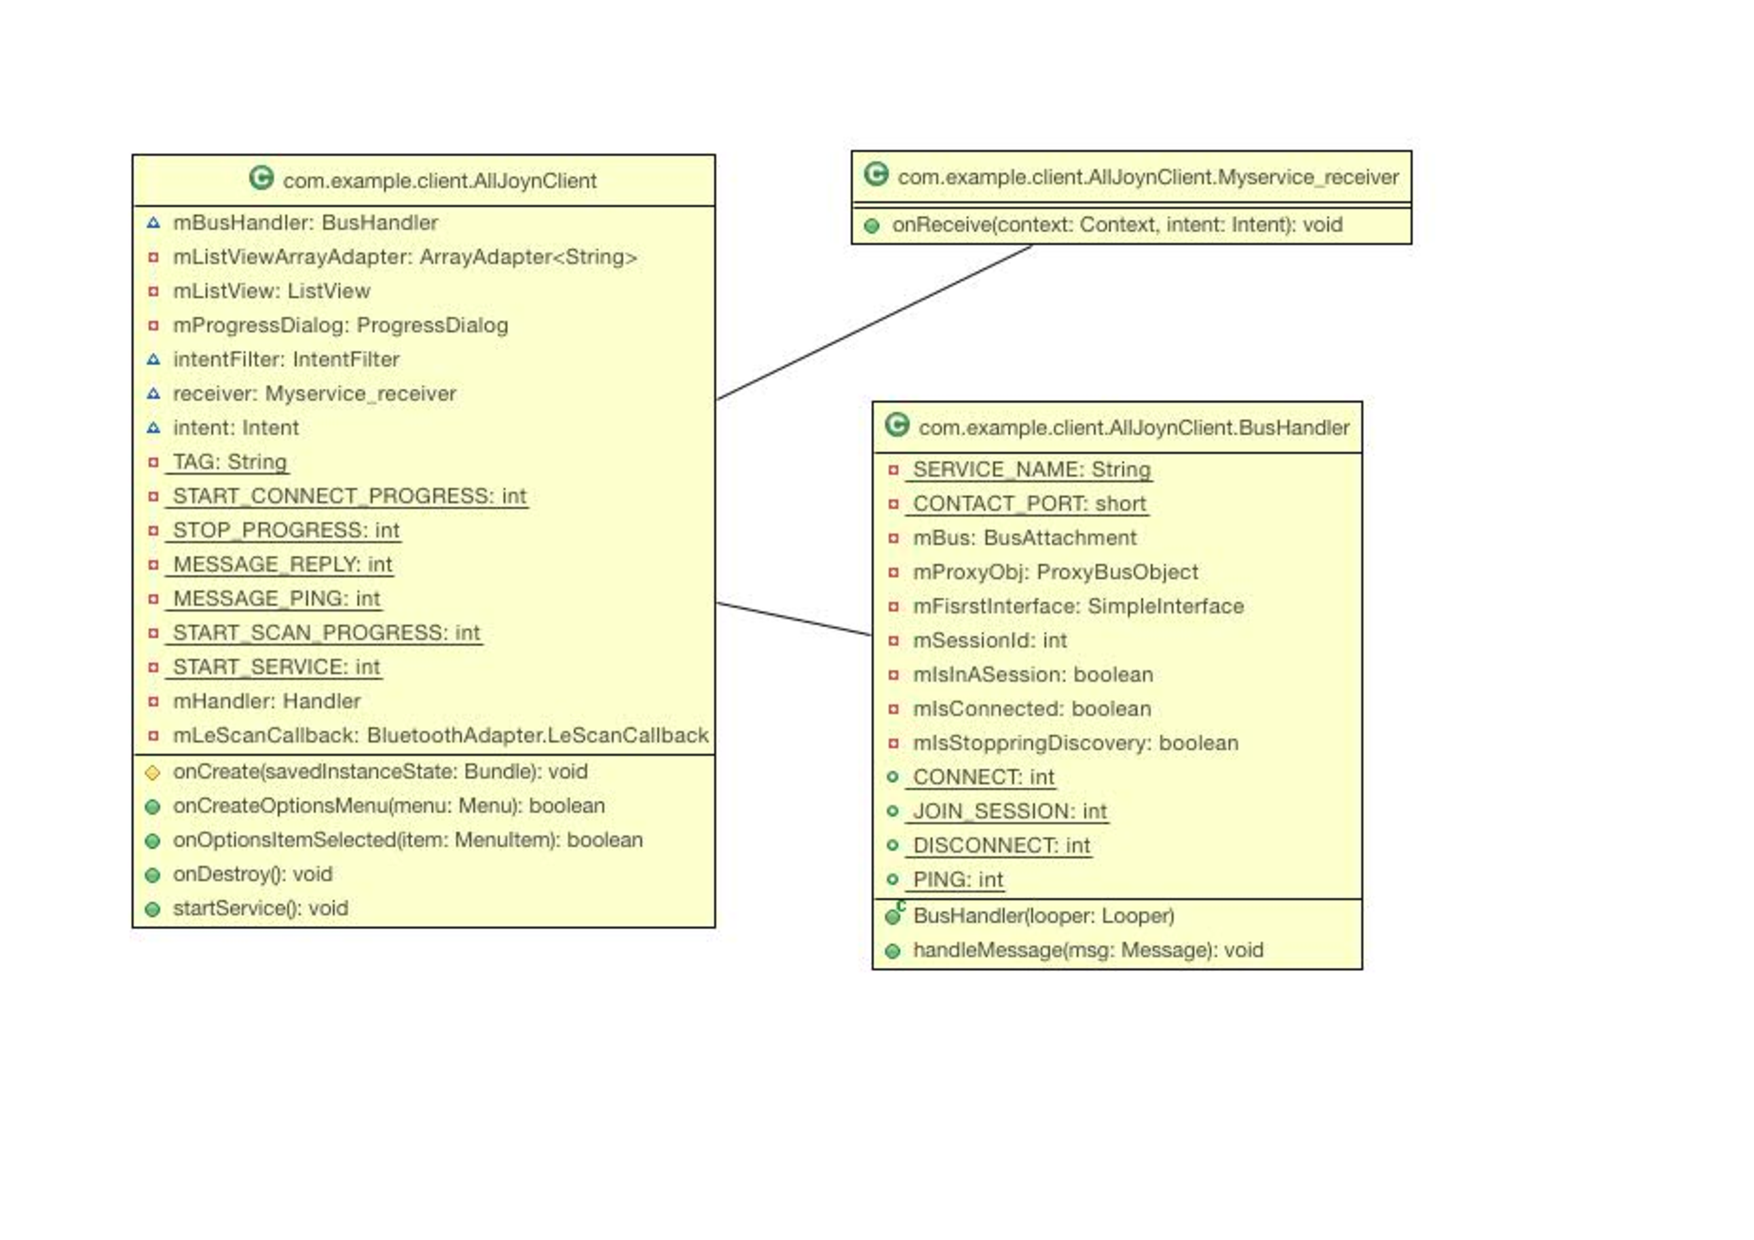
\includegraphics[width=10cm]{fig/class_client.pdf}
\end{center}
\caption{AllJoynClientクラス図}
\end{minipage}
\begin{minipage}{0.5 \hsize}
\begin{center}
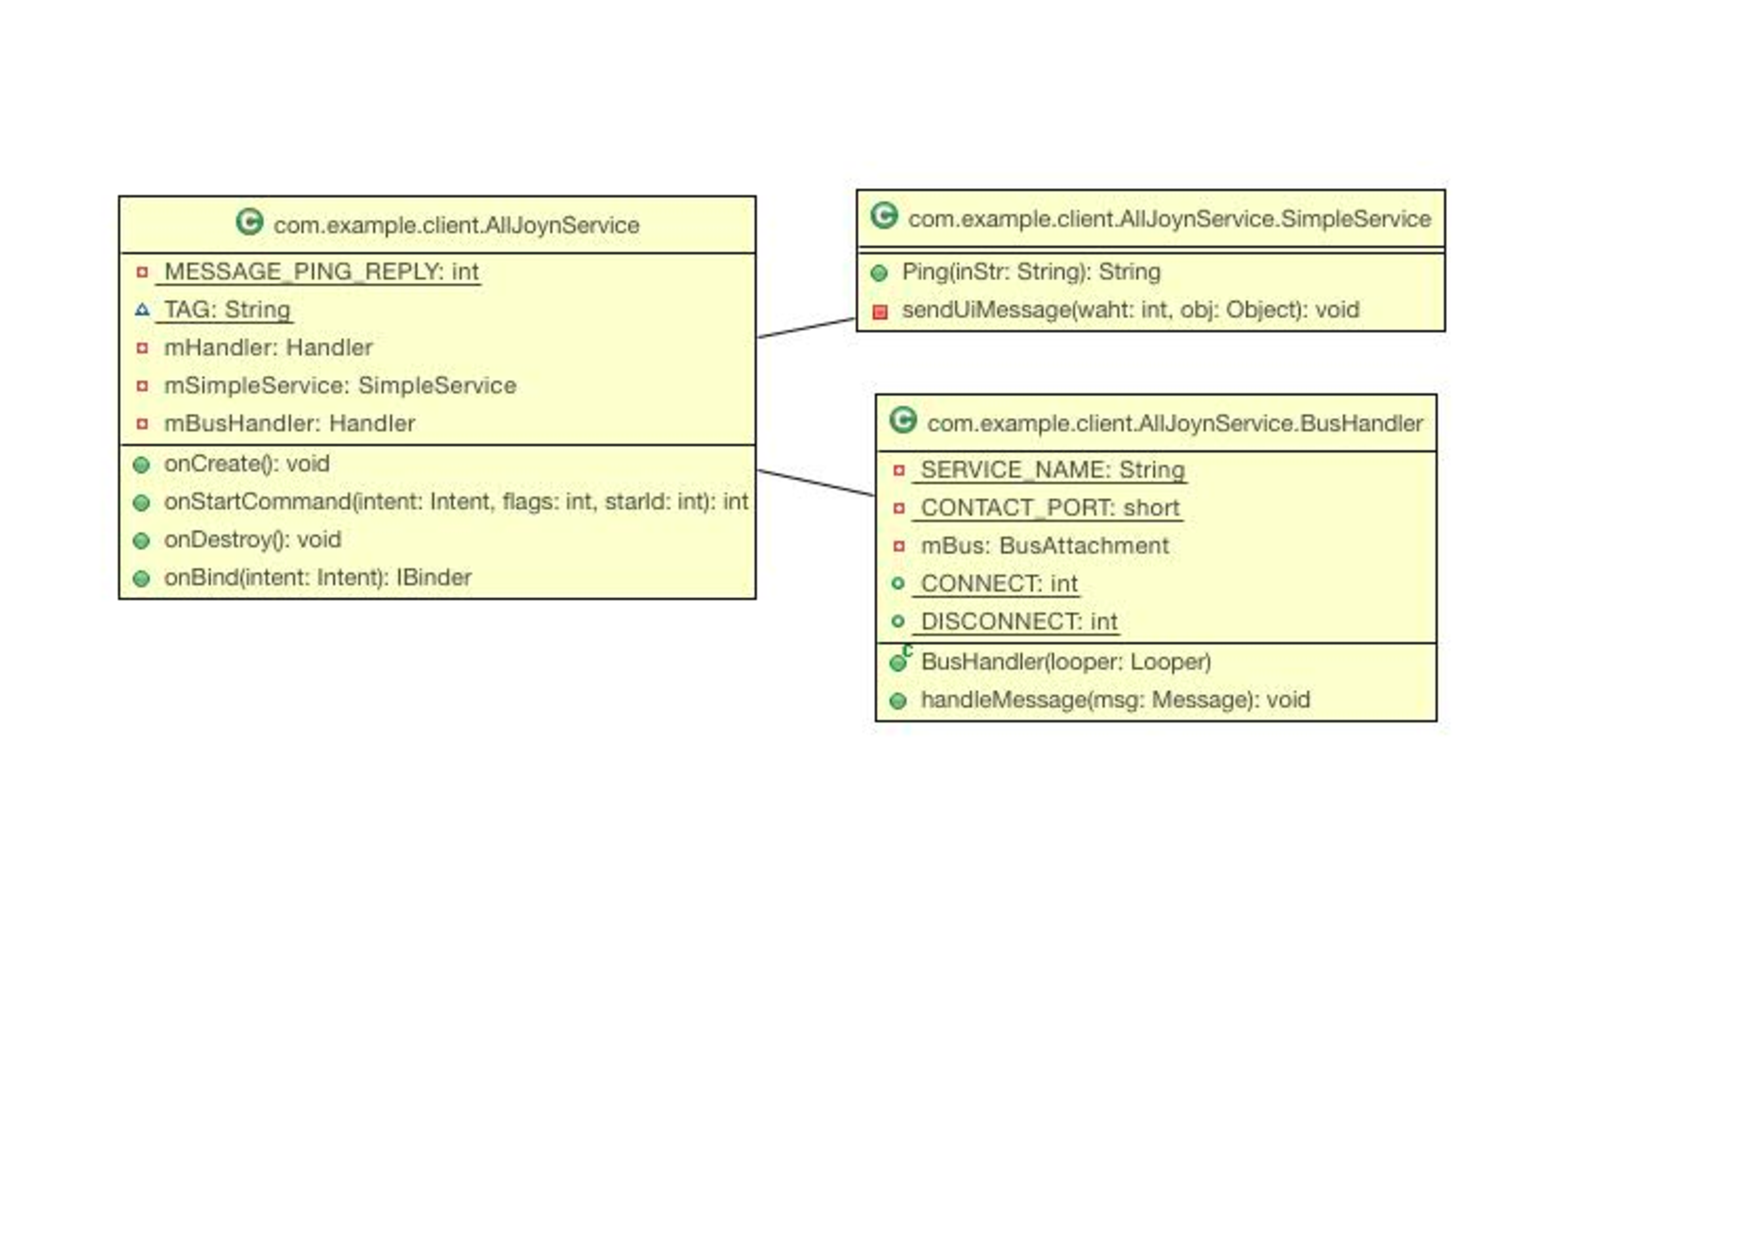
\includegraphics[width=10cm]{fig/class_service.pdf}
\end{center}
\caption{AllJoynServiceクラス図}
\end{minipage}
\end{figure}

\begin{figure}[htbp]
\centering
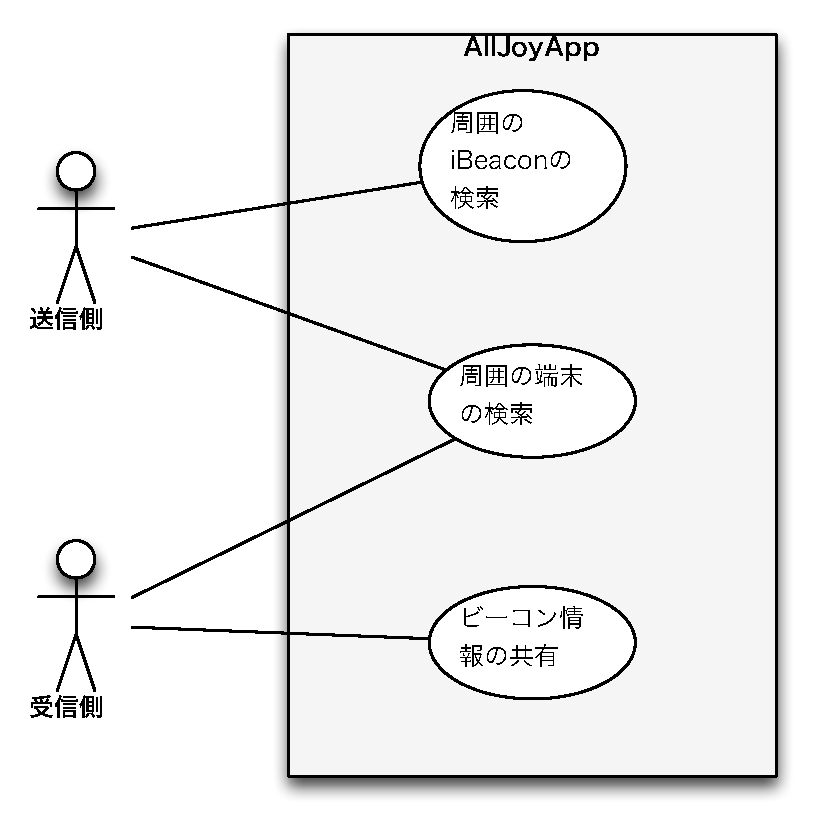
\includegraphics[width=7cm]{fig/usecase.pdf}
\caption{ユースケース図}
\end{figure}

\subsection{アプリケーションの起動}
今回作成したAllJoynAppを起動すると,AllJoynClientとAllJoynServiceの二つが起動する.
AllJoynClientは画面上にFIND,SCANという二つのボタンを表示する.
AllJoynServiceはAllJoyn Routerと接続し,周囲のAllJoyn RouterにAdvertiseする.

\begin{figure}[htbp]
\centering
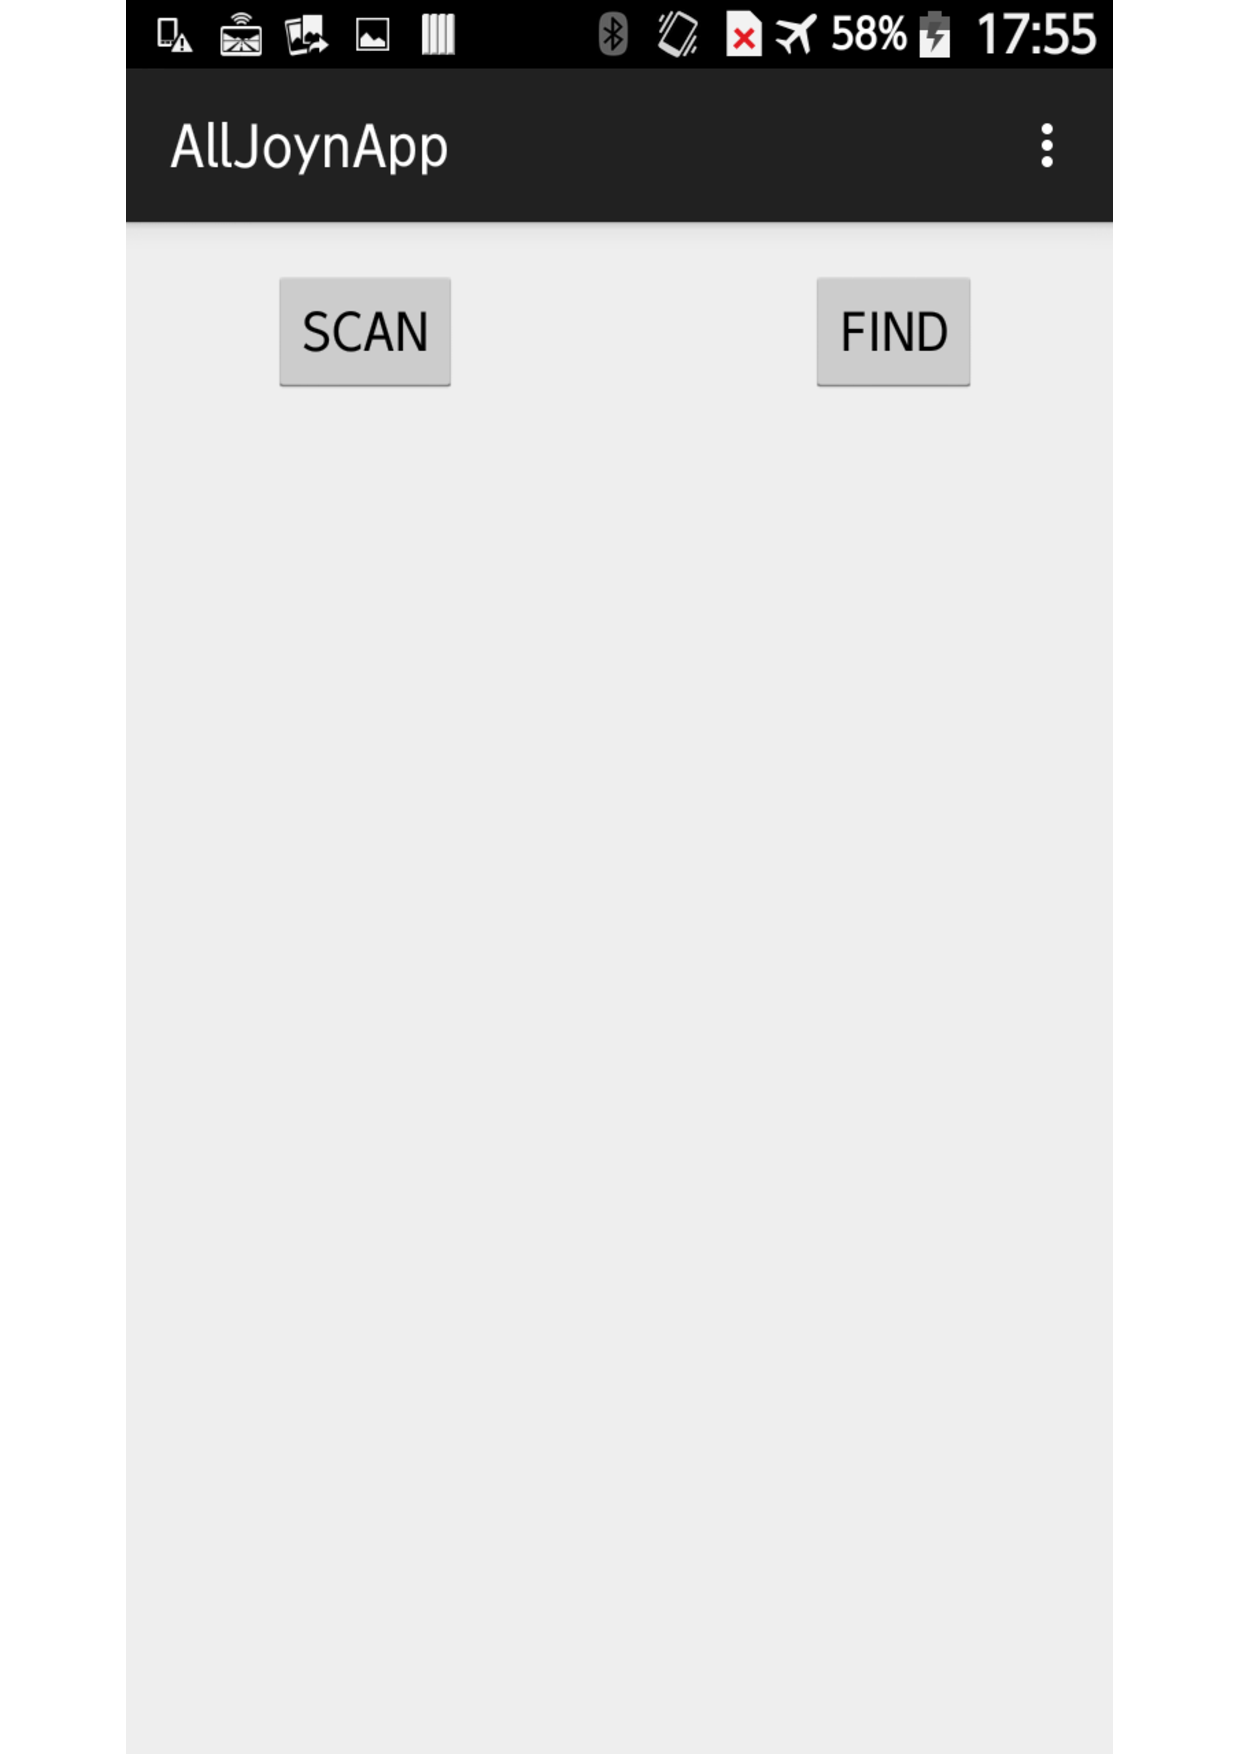
\includegraphics[width=5cm]{fig/screen1.pdf}
\caption{アプリケーション起動画面}
\end{figure}

\begin{figure}[htbp]
\centering
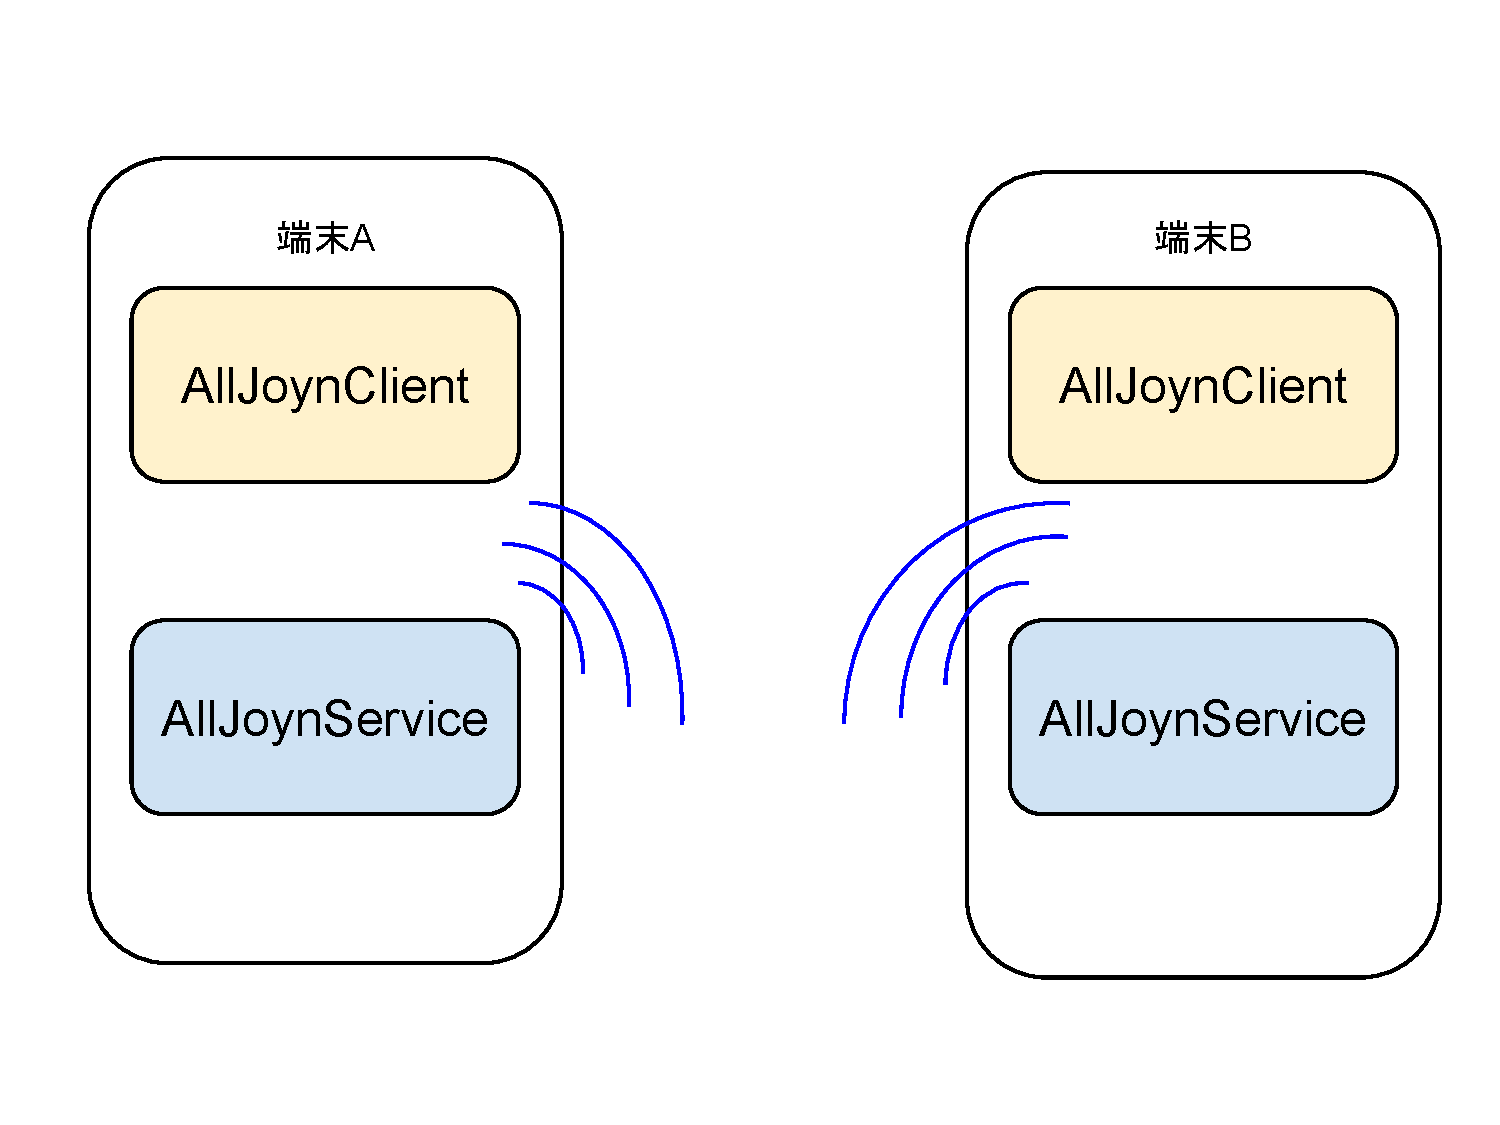
\includegraphics[width=10cm]{fig/appstart.pdf}
\caption{アプリケーション起動画面}
\end{figure}


\subsection{FINDボタン押下}
FINDボタンを押下した際の処理は以下の通りである.

\begin{enumerate}
\item 自身のAllJoynServiceを停止する.
\item AllJoynClientは自身のAllJoynRouterと接続する
\item 周囲のAllJoynServiceをDiscoveryする.
\item 検索している間,画面上には'DISCOVERING'と表示される
\item AllJoynServiceを検知した場合,コネクションを確立し,'DISCOVERING'の表示をやめる.
\end{enumerate}

\begin{figure}[htbp]
\centering
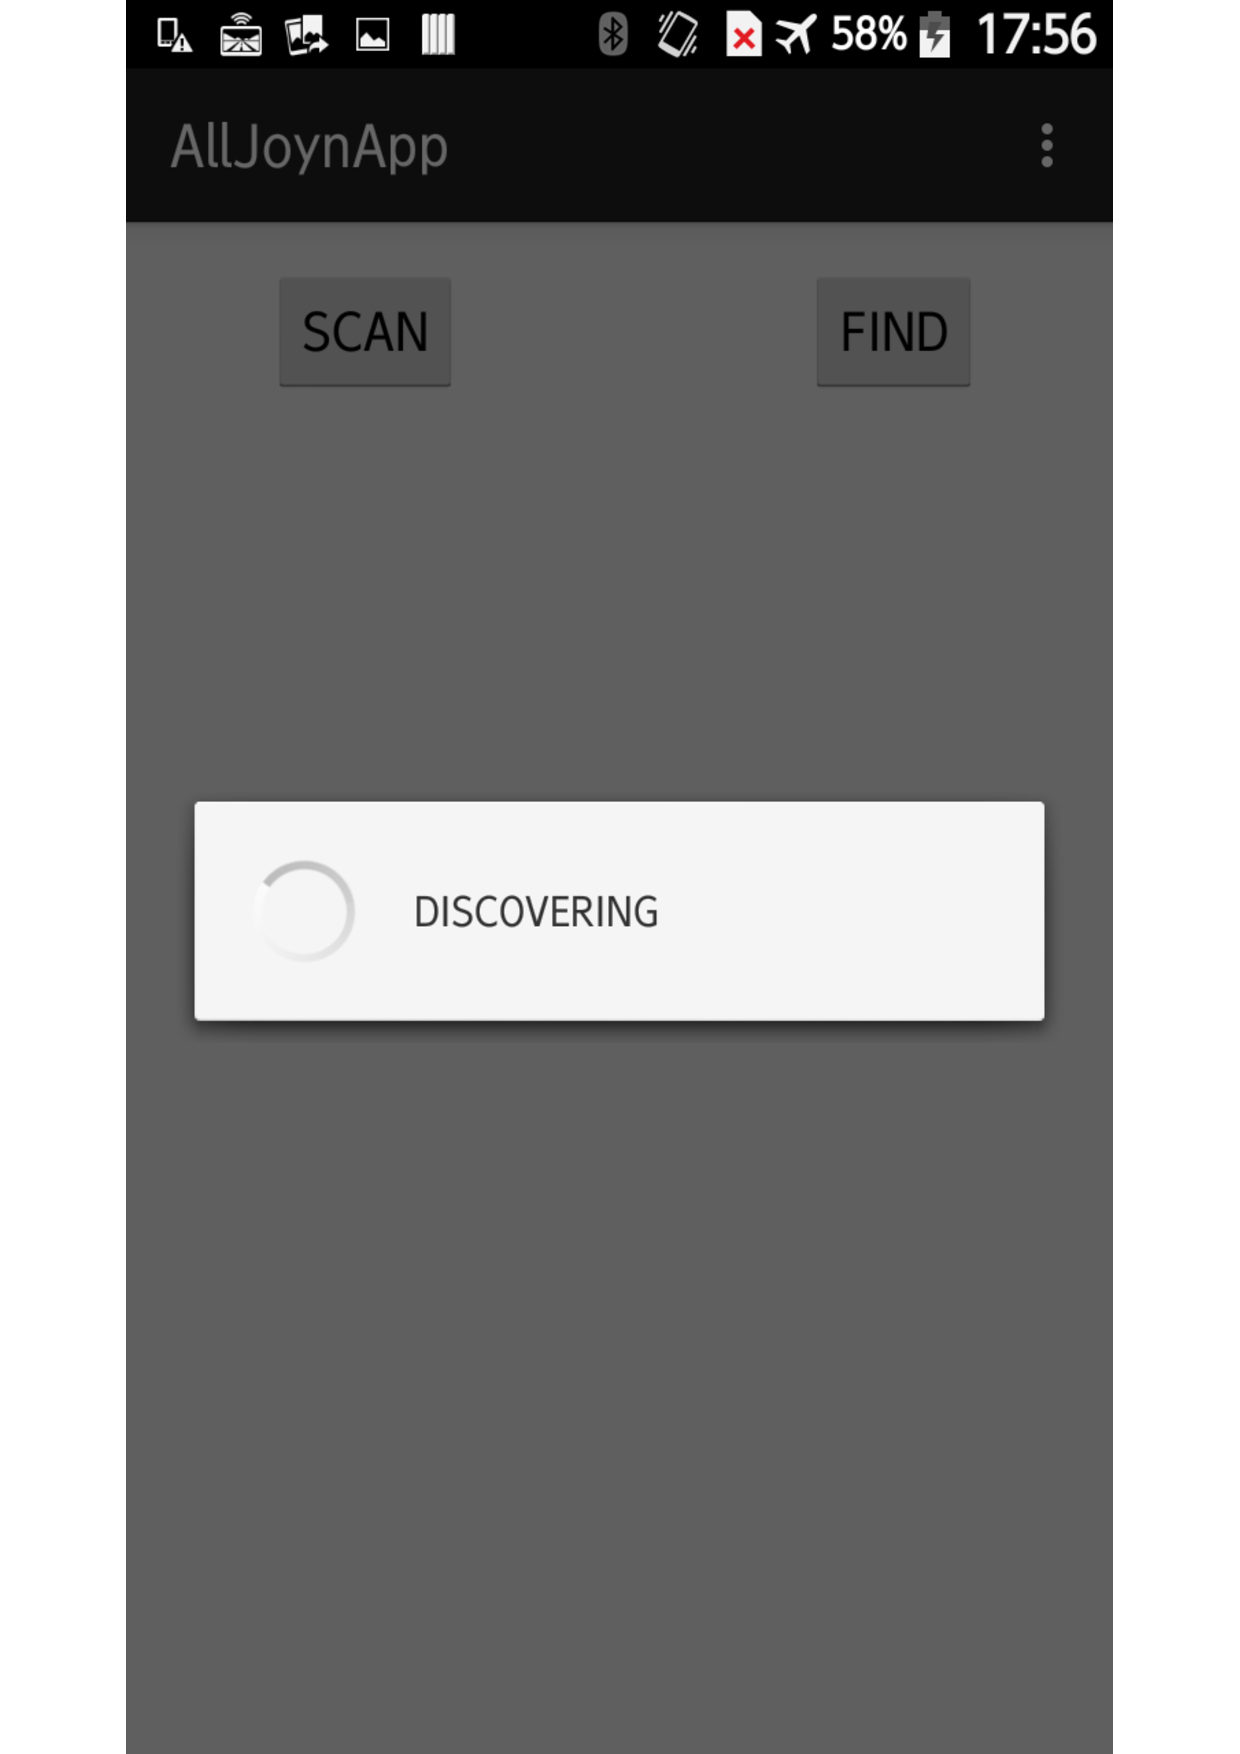
\includegraphics[width=5cm]{fig/screen2.pdf}
\caption{FINDボタン押下}
\end{figure}

\subsection{SCANボタン押下}
SCANボタンが押下された際の処理は以下の通りである.
\begin{enumerate}
\item 二秒間周囲のビーコンを検知し,ビーコン情報を画面上に表示する.
\item AllJoynClientから,自身と接続されているAllJoynServiceにビーコン情報を送信する.
\item AllJoynServiceは受信したビーコン情報を画面上に表示する.
\item 自身のAllJoynServiceを起動する.
\end{enumerate}

\begin{figure}[htbp]
\centering
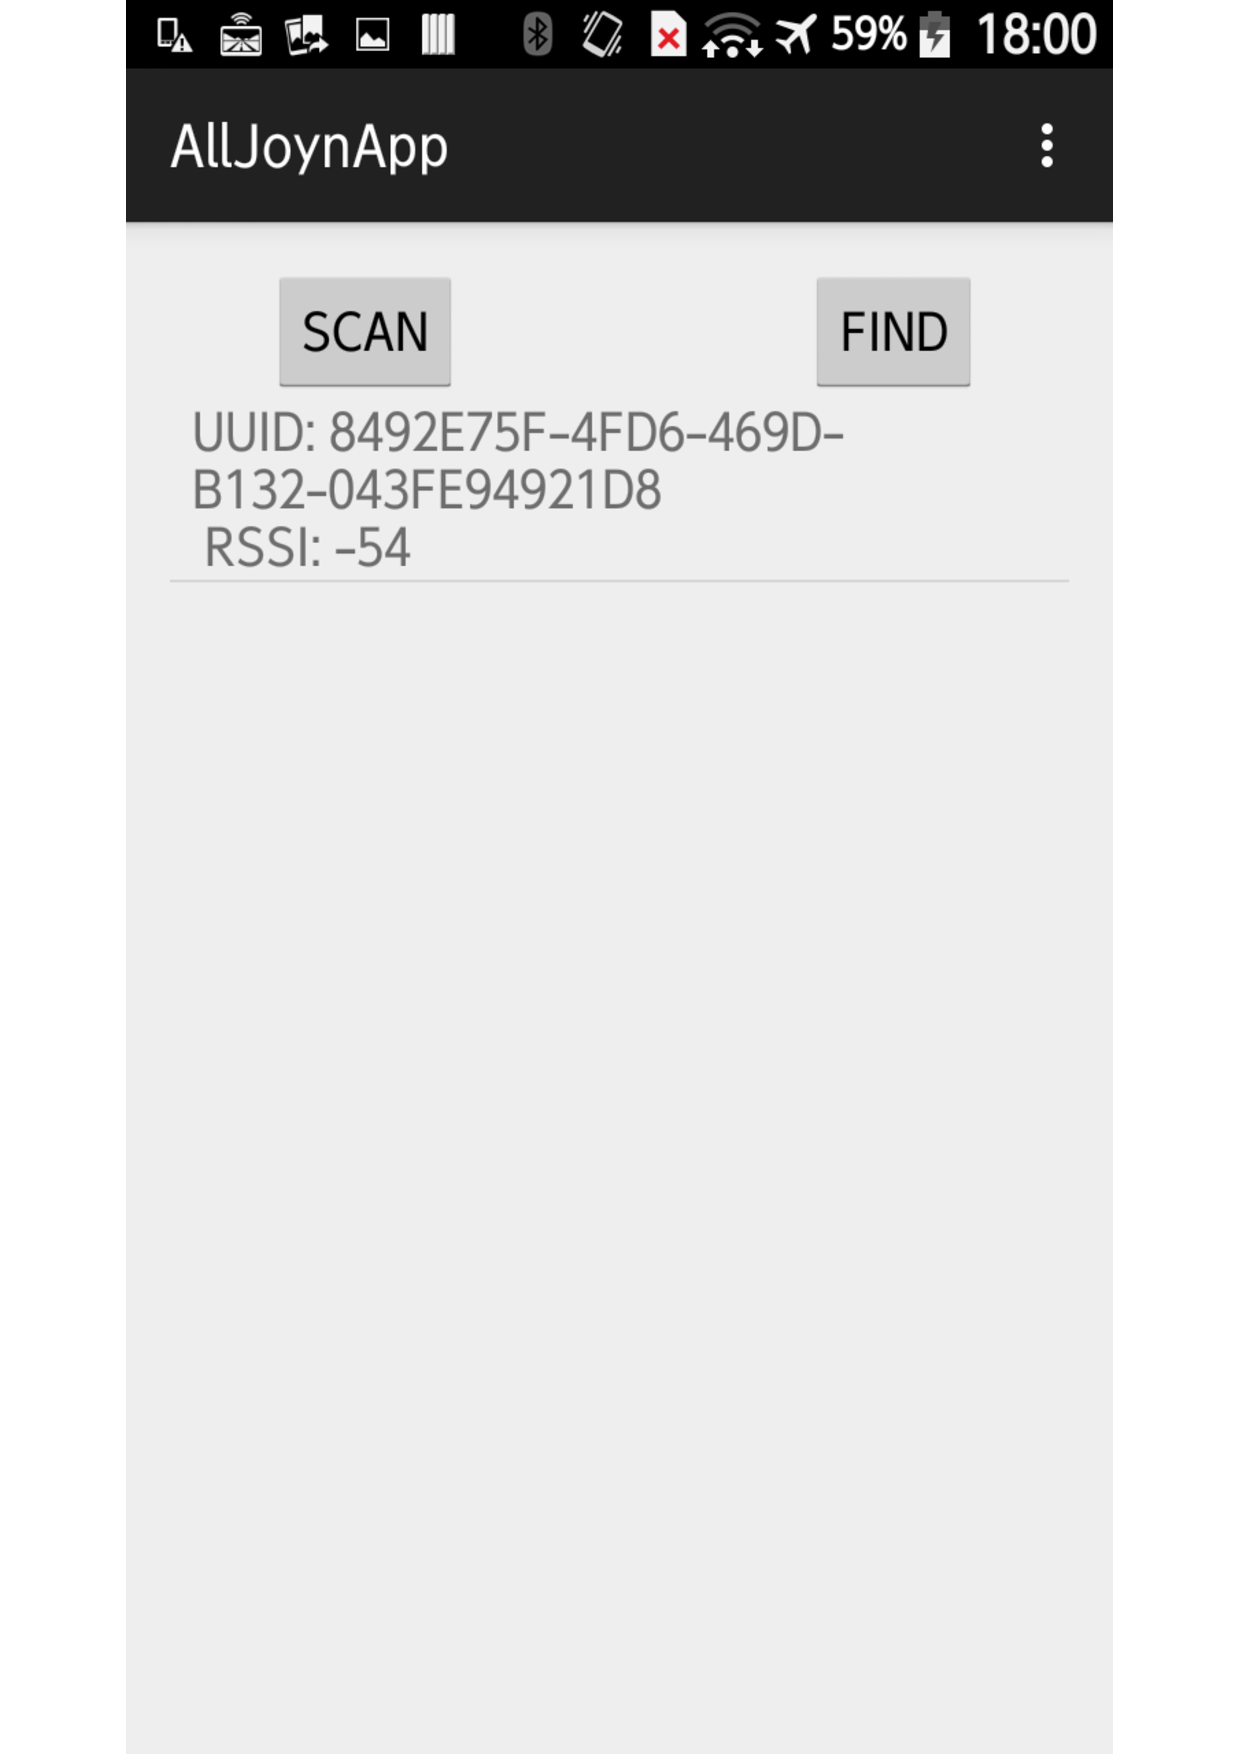
\includegraphics[width=5cm]{fig/screen3.pdf}
\caption{SCANボタン押下}
\end{figure}


\section{考察}
